\documentclass[Main]{subfiles}
\begin{document}

\chapter{Conclusion}

\section{Conclusion}
Java RMI (Remote Method Invocation) can be used to invoke methods of
objects in another Java Virtual Machine (JVM). The JVM can be on the
local host or another host. RMI allows the client to invoke remote methods in the server as if the remote object were contained on the client host, from the programmer's perspective.\\When a client calls a method in a remote object, instead of letting the Java runtime take care of the call as it would for regular Java objects, the RMI runtime system takes over and routes the call over the network to the remote object. None of the underlying communication is visible to the programmer.


\section{Discussion}

Maybe we can use some of this to argue why to use Java RMI:
\begin{figure}[H]
\centering
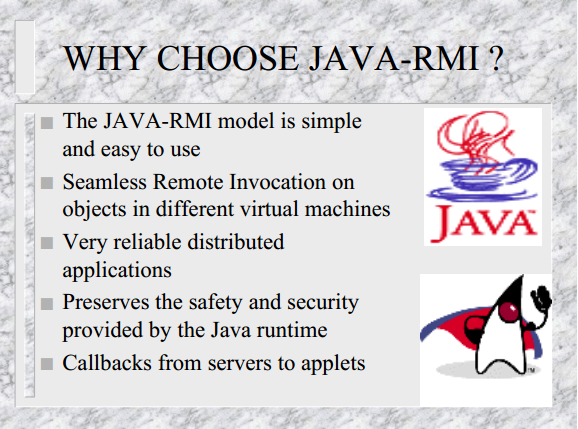
\includegraphics[scale=1]{Figurer/discussion.png}
\caption{From: http://www.uniforum.chi.il.us/slides/javarmi/javarmi.pdf}
\end{figure}


\section{Perspectives}
What are the perspectives on the technology and your prototype? 


\end{document} 